\chapter{Analysis}

\section{Chapter content}
In this chapter I will present the results of my analysis.\\
-Describe quantifiers and discuss the results of analysing the experimental recordings\\
-image of table containing everything the jupyter notebook has computed\\
-table with info on electrical frequency levels in each recording\\
-diagram showing a quantifier (peak firing frequency) and electrical frequency for each spike train of single recording\\
-compare diagrams of different recordings\\
-compare different quantifiers in one diagram with each other for the same file\\
-compare ISI to log(ISI) for every train in one file\\

\section{}
-Show picture of a table with all the quantifiers as an example and add the rest to the appendix\\
\begin{figure}
	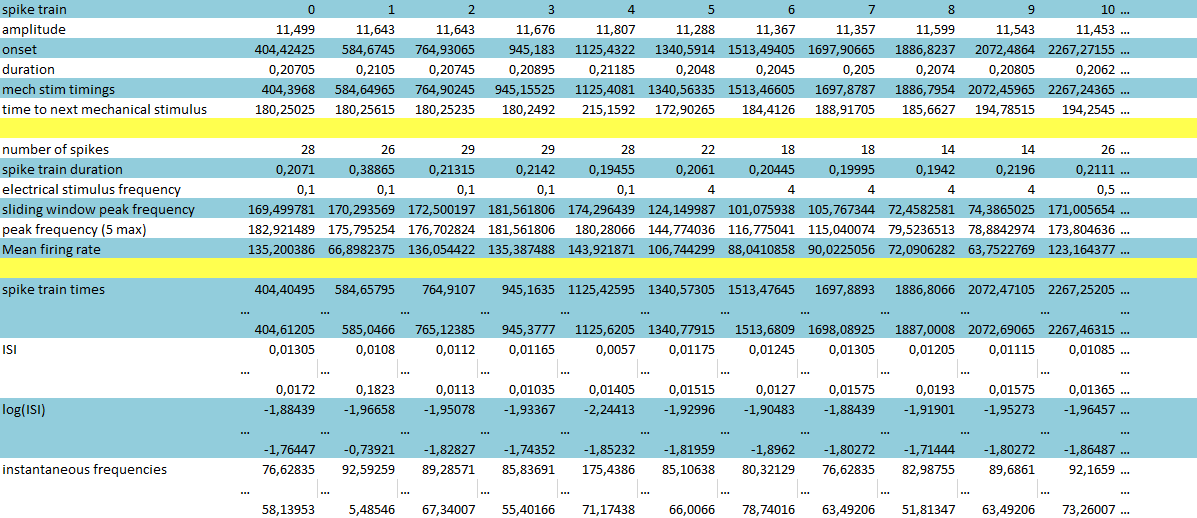
\includegraphics[width = \textwidth]{src/pic/sc_table}
	\caption{Sample picture of table after successful analysis }
	\label{fig:table_sc}
\end{figure}
-first batch contains information on the mechanical stimulus, second batch single number quantifiers about spike train, last batch lists of raw data and list quantifiers such as ISI\\
-with the help of this diagram describe the quantifiers and results that were computed\\


%selected additional information in more detail:

%-diagram of peak firing frequency, spike counts, train duration and electrical frequency\\
%-shows the correlation between electrical frequency and the other quantifiers of single spike trains\\

%-diagrams of Interspike Intervals(isi) and logarithm of isi\\
%-should show that by taking the logarithm, the isi becomes more linear\\




\cleardoublepage
